% bab5.tex - Hasil dan Pembahasan (Sesi B, L4-L5).
% Aturan: semua angka kinerja berasal dari tabel/*.tex dan makro tabel/angka.tex yang dibuat
% skrip/tabel_ke_tex.py dari bench/results/*.csv; JANGAN mengetik angka kinerja di berkas ini.
% Satu tabel satu mesin; data sintetis selalu ditandai; total_ms tanpa pemanasan CUDA, Proses dengan pemanasan.
\chapter{HASIL DAN PEMBAHASAN}

\section{Lingkungan dan Data Uji}
\label{sec:lingkungan}
Pengukuran dilakukan di tiga komputer anggota kelompok (Tabel~\ref{tab:mesin}). Agar angka tidak tercampur, setiap tabel di bab ini hanya memuat hasil dari satu mesin. Seluruh angka kinerja utama berasal dari Mesin B. Mesin A hanya dipakai untuk profil L0 sebagai pembanding, sedangkan Mesin C dipakai untuk uji fungsional aplikasi dengan citra Sentinel-2.

\begin{table}[H]
\centering
\caption{Mesin uji dan eksperimen yang dijalankan di masing-masing mesin}
\label{tab:mesin}
\small
\begin{tabularx}{\textwidth}{L{1.6cm}YY}
\hline
\hdr{Mesin} & \hdr{Spesifikasi} & \hdr{Eksperimen} \\ \hline
A & Intel Core i7-1065G7 (4 inti, 8 \emph{thread}), RAM 16 GB; WSL 2, GCC 11.4 & Profil L0 (Tabel~\ref{tab:l0a}), hanya sebagai pembanding \\ \hline
B & Intel Core i7-13620H (16 CPU logis di WSL), NVIDIA RTX 3050 6 GB Laptop (\kode{sm\_86}, \emph{driver} 576.93), RAM WSL 7,6 GiB; WSL 2 Ubuntu 24.04, CUDA 12.9, GCC 13.3; skema daya \emph{Balanced} & Semua \emph{benchmark} kinerja: per tahap, optimasi bertahap, \emph{strong}/\emph{weak scaling}, varian CUDA, ambang mode otomatis \\ \hline
C & Intel Core i7-13650HX, NVIDIA RTX 3050 6 GB Laptop; WSL 2 Ubuntu 24.04 & Uji fungsional Sentinel-2, verifikasi \kode{cmp}, tangkapan layar aplikasi. Waktunya bukan hasil kinerja resmi \\ \hline
\end{tabularx}
\par\smallskip\footnotesize\raggedright Sumber: \kode{bench/results/run\_20261127\_1634\_env.txt} dan \kode{bench/BENCH\_GPU.md} (B), \kode{docs/PROFIL\_L0.md} (A), \kode{meta.json} \emph{run} Sentinel-2 (C).
\end{table}

\textbf{Data uji.} Ada dua jenis citra:
\begin{itemize}
    \item \textbf{Citra sintetis} (\kode{sintetis\_lanskap\_\textless lebar\textgreater x\textless tinggi\textgreater}) yang dibangkitkan skrip \emph{benchmark}, berukuran 1000$\times$1000, 2000$\times$2000, 4000$\times$3000, dan 7680$\times$4320 piksel untuk pengukuran utama; 320$\times$320 sampai 4000$\times$3000 untuk penentuan ambang; dan 2000$\times$1000 sampai 32000$\times$1000 untuk \emph{weak scaling}. Varian CUDA diukur pada citra acak. \textbf{Semua angka kinerja di Subbab~\ref{sec:profil} sampai~\ref{sec:hasilambang} berasal dari citra sintetis.}
    \item \textbf{Citra Sentinel-2} \emph{tile} T49MDM (\kode{S2B\_MSIL2A\_20261017}), kanal B04/B03/B02, berupa potongan 512, 1024, dan 2048 piksel persegi. Citra ini dipakai untuk uji fungsional dan verifikasi (Subbab~\ref{sec:hasilverifikasi} dan~\ref{sec:hasilsentinel}).
\end{itemize}

\textbf{Prosedur.} Setiap konfigurasi dijalankan satu kali sebagai pemanasan (dibuang), lalu lima kali; yang dilaporkan adalah median. Semua \emph{run} memakai 20 iterasi dan \emph{seed} 42. Waktu diambil dari \kode{timing.json} keluaran \kode{landcover} (Subbab~\ref{sec:kontrak}). \textbf{Total} adalah \kode{total\_ms}, yaitu baca + K-Means + pewarnaan + tulis, tanpa pemanasan konteks CUDA. \textbf{Proses} adalah waktu dinding satu proses \kode{landcover} (\kode{wall\_ms}) yang mencakup pemanasan itu. Keduanya disajikan karena aplikasi menjalankan \kode{landcover} sebagai proses baru di setiap \emph{run}, sehingga pengguna merasakan Proses, bukan Total. Pada sesi Mesin B yang merekamnya (\emph{run} 16:34 dan sesi ambang), pemanasan konteks CUDA berkisar \WarmMin--\WarmMax~ms per proses.

\textbf{Penyimpangan dari rencana proposal.}
\begin{enumerate}
    \item Median dari 5 ulangan, bukan minimal 10.
    \item Ukuran citra 1000$^2$, 2000$^2$, 4000$\times$3000, dan 7680$\times$4320, bukan 2048$^2$, 4096$^2$, 8192$^2$, dan satu \emph{tile} penuh. \emph{Tile} penuh 10980$\times$10980 tidak tersedia (Subbab~\ref{sec:batasan}).
    \item \emph{Profiling} memakai pengukur waktu per tahap di dalam program dan CUDA \emph{events}, bukan \kode{perf}/\kode{gprof}; Nsight (\kode{nsys}/\kode{ncu}) tidak terpasang di mesin uji.
    \item Mesin uji adalah laptop anggota kelompok (Tabel~\ref{tab:mesin}), bukan mesin pada rencana proposal.
    \item Tahap baca PNG tetap serial di semua mode (Tabel~\ref{tab:penempatan}).
\end{enumerate}

\section{Profiling L0 dan \emph{Bottleneck}}
\label{sec:profil}
Tabel~\ref{tab:l0b} menunjukkan waktu setiap tahap pada mode CPU saja (L0, \kode{kmeans\_cpu} satu \emph{thread}) di Mesin B. Pada semua ukuran dan nilai $K$ yang diukur, K-Means adalah tahap terbesar dengan porsi \PorsiKMLoMin--\PorsiKMLoMax{} dari Total. Porsinya membesar seiring $K$, karena biaya \emph{assignment} sebanding dengan $N\times K$, sedangkan baca dan tulis PNG hanya bergantung pada jumlah piksel dan isi citra. Tahap inisialisasi praktis nol karena hanya memilih $K$ \emph{centroid} awal.

% DIBUAT OLEH laporan/skrip/tabel_ke_tex.py -- jangan disunting tangan.
\begin{table}[H]
\centering
\caption{Waktu per tahap mode CPU saja (L0) dan porsi K-Means, citra sintetis, Mesin B (ms)}
\label{tab:l0b}
\small
\begin{tabularx}{\textwidth}{L{2.3cm}r>{\raggedleft\arraybackslash}X>{\raggedleft\arraybackslash}X>{\raggedleft\arraybackslash}X>{\raggedleft\arraybackslash}X>{\raggedleft\arraybackslash}X>{\raggedleft\arraybackslash}X>{\raggedleft\arraybackslash}X}
\hline
\hdr{Citra} & \hdr{$K$} & \hdr{Baca} & \hdr{Init} & \hdr{K-Means} & \hdr{Warna} & \hdr{Tulis} & \hdr{Total} & \hdr{Porsi K-Means} \\ \hline
4000$\times$3000 & 2 & 167,2 & 0,0 & 640,7 & 10,0 & 50,4 & 875,1 & 73\% \\ \hline
4000$\times$3000 & 4 & 156,1 & 0,0 & 1017,2 & 9,6 & 51,9 & 1224,8 & 83\% \\ \hline
1000$\times$1000 & 8 & 13,2 & 0,0 & 207,5 & 0,7 & 17,4 & 237,4 & 87\% \\ \hline
2000$\times$2000 & 8 & 52,9 & 0,0 & 777,4 & 4,0 & 85,8 & 921,7 & 84\% \\ \hline
4000$\times$3000 & 8 & 161,5 & 0,0 & 2385,1 & 11,8 & 215,2 & 2750,3 & 87\% \\ \hline
7680$\times$4320 & 8 & 431,3 & 0,0 & 5870,6 & 24,0 & 419,3 & 6765,7 & 87\% \\ \hline
4000$\times$3000 & 16 & 170,7 & 0,0 & 4794,6 & 13,8 & 417,7 & 5400,7 & 89\% \\ \hline
\end{tabularx}
\par\smallskip\footnotesize\raggedright Median 5 ulangan setelah 1 pemanasan, 20 iterasi, \emph{seed} 42. Sumber: \kode{bench\_gpu\_summary.csv} dan \kode{run\_20261127\_1634\_ksweep\_summary.csv} (4000$\times$3000 dari \emph{run} 16:34).
\end{table}


Pola yang sama muncul di Mesin A (Tabel~\ref{tab:l0a}): porsi K-Means \PorsiKMAMin--\PorsiKMAMax. Waktu mutlak kedua mesin berbeda dan tidak dibandingkan. Yang penting adalah kesimpulannya sama di dua mesin: K-Means adalah \emph{bottleneck} utama L0, sehingga menjadi sasaran pertama L1 (CUDA) dan L2 (OpenMP). Sesudah K-Means, tahap berikutnya yang terbesar adalah tulis dan baca PNG.

% DIBUAT OLEH laporan/skrip/tabel_ke_tex.py -- jangan disunting tangan.
\begin{table}[H]
\centering
\caption{Pembanding: waktu per tahap L0 di Mesin A (i7-1065G7), citra sintetis (ms)}
\label{tab:l0a}
\small
\begin{tabularx}{\textwidth}{L{2.3cm}r>{\raggedleft\arraybackslash}X>{\raggedleft\arraybackslash}X>{\raggedleft\arraybackslash}X>{\raggedleft\arraybackslash}X>{\raggedleft\arraybackslash}X>{\raggedleft\arraybackslash}X>{\raggedleft\arraybackslash}X}
\hline
\hdr{Citra} & \hdr{$K$} & \hdr{Baca} & \hdr{Init} & \hdr{K-Means} & \hdr{Warna} & \hdr{Tulis} & \hdr{Total} & \hdr{Porsi K-Means} \\ \hline
1000$\times$1000 & 8 & 19,0 & 0,0 & 313,9 & 0,9 & 42,8 & 375,1 & 84\% \\ \hline
2000$\times$2000 & 8 & 67,0 & 0,0 & 1038,5 & 3,3 & 214,0 & 1322,8 & 79\% \\ \hline
4000$\times$3000 & 8 & 201,0 & 0,0 & 3084,7 & 10,1 & 521,2 & 3827,2 & 81\% \\ \hline
7680$\times$4320 & 8 & 569,4 & 0,0 & 8483,4 & 29,1 & 1198,9 & 10263,9 & 83\% \\ \hline
4000$\times$3000 & 4 & 206,4 & 0,0 & 1514,7 & 9,9 & 267,4 & 2002,5 & 76\% \\ \hline
4000$\times$3000 & 16 & 208,6 & 0,0 & 6556,9 & 10,8 & 1073,6 & 7871,4 & 83\% \\ \hline
\end{tabularx}
\par\smallskip\footnotesize\raggedright Median 5 ulangan setelah 1 pemanasan. Sumber: \kode{docs/PROFIL\_L0\_tabel.md} (\kode{bench/profile\_l0.py}). Mesin berbeda dengan tabel lain di bab ini; angkanya tidak dibandingkan langsung dengan Mesin B.
\end{table}


\section{Optimasi Bertahap}
\label{sec:bertahap}
Tabel~\ref{tab:bertahapk8} membandingkan langkah optimasi pada $K=8$ untuk empat ukuran citra. Untuk L2 dan L1+L2, yang ditampilkan adalah jumlah \emph{thread} OpenMP dengan Total terkecil. Gambar~\ref{fig:tahap} menampilkan komposisi tahap pada citra terbesar.

% DIBUAT OLEH laporan/skrip/tabel_ke_tex.py -- jangan disunting tangan.
\begin{table}[H]
\centering
\caption{Optimasi bertahap L0 $\rightarrow$ L2 $\rightarrow$ L1 $\rightarrow$ L1+L2, $K=8$, citra sintetis, Mesin B (ms; $S$ = \emph{speedup} terhadap L0)}
\label{tab:bertahapk8}
\footnotesize
\begin{tabularx}{\textwidth}{L{2.1cm}rL{2.3cm}>{\raggedleft\arraybackslash}X>{\raggedleft\arraybackslash}X>{\raggedleft\arraybackslash}X>{\raggedleft\arraybackslash}X>{\raggedleft\arraybackslash}X>{\raggedleft\arraybackslash}X}
\hline
\hdr{Citra} & \hdr{$K$} & \hdr{Konfigurasi} & \hdr{K-Means} & \hdr{$S$ K-Means} & \hdr{Total} & \hdr{$S$ Total} & \hdr{Proses} & \hdr{$S$ Proses} \\ \hline
1000$\times$1000 & 8 & L0 & 207,5 & 1,0\ensuremath{\times} & 237,4 & 1,00\ensuremath{\times} & -- & -- \\ \hline
1000$\times$1000 & 8 & L2 (8 thr) & 43,5 & 4,8\ensuremath{\times} & 73,7 & 3,22\ensuremath{\times} & -- & -- \\ \hline
1000$\times$1000 & 8 & L1 & 4,8 & 42,9\ensuremath{\times} & 37,4 & 6,35\ensuremath{\times} & -- & -- \\ \hline
1000$\times$1000 & 8 & L1+L2 (2 thr) & 5,1 & 40,6\ensuremath{\times} & 34,5 & 6,89\ensuremath{\times} & -- & -- \\ \hline
2000$\times$2000 & 8 & L0 & 777,4 & 1,0\ensuremath{\times} & 921,7 & 1,00\ensuremath{\times} & -- & -- \\ \hline
2000$\times$2000 & 8 & L2 (8 thr) & 165,0 & 4,7\ensuremath{\times} & 245,1 & 3,76\ensuremath{\times} & -- & -- \\ \hline
2000$\times$2000 & 8 & L1 & 18,5 & 41,9\ensuremath{\times} & 159,5 & 5,78\ensuremath{\times} & -- & -- \\ \hline
2000$\times$2000 & 8 & L1+L2 (4 thr) & 17,9 & 43,4\ensuremath{\times} & 112,7 & 8,18\ensuremath{\times} & -- & -- \\ \hline
4000$\times$3000 & 8 & L0 & 2385,1 & 1,0\ensuremath{\times} & 2750,3 & 1,00\ensuremath{\times} & 2800,7 & 1,00\ensuremath{\times} \\ \hline
4000$\times$3000 & 8 & L2 (16 thr) & 337,3 & 7,1\ensuremath{\times} & 560,7 & 4,90\ensuremath{\times} & 617,2 & 4,54\ensuremath{\times} \\ \hline
4000$\times$3000 & 8 & L1 & 55,7 & 42,8\ensuremath{\times} & 436,2 & 6,31\ensuremath{\times} & 720,3 & 3,89\ensuremath{\times} \\ \hline
4000$\times$3000 & 8 & L1+L2 (8 thr) & 55,4 & 43,1\ensuremath{\times} & 291,9 & 9,42\ensuremath{\times} & 600,7 & 4,66\ensuremath{\times} \\ \hline
7680$\times$4320 & 8 & L0 & 5870,6 & 1,0\ensuremath{\times} & 6765,7 & 1,00\ensuremath{\times} & -- & -- \\ \hline
7680$\times$4320 & 8 & L2 (8 thr) & 1258,0 & 4,7\ensuremath{\times} & 1875,9 & 3,61\ensuremath{\times} & -- & -- \\ \hline
7680$\times$4320 & 8 & L1 & 138,9 & 42,3\ensuremath{\times} & 1033,1 & 6,55\ensuremath{\times} & -- & -- \\ \hline
7680$\times$4320 & 8 & L1+L2 (16 thr) & 131,8 & 44,6\ensuremath{\times} & 684,1 & 9,89\ensuremath{\times} & -- & -- \\ \hline
\end{tabularx}
\par\smallskip\footnotesize\raggedright L2 dan L1+L2: konfigurasi terbaik menurut Total; ``thr'' = jumlah \emph{thread} OpenMP. Total = \kode{total\_ms}, tanpa pemanasan konteks CUDA. Proses = waktu dinding satu proses \kode{landcover} (\kode{wall\_ms}), termasuk pemanasan. ``--'' = tidak diukur: sesi \kode{bench\_gpu} (1000$^2$, 2000$^2$, 7680$\times$4320) belum merekam \kode{wall\_ms}; baris 4000$\times$3000 dari \emph{run} 16:34.
\end{table}


\begin{figure}[H]
\centering
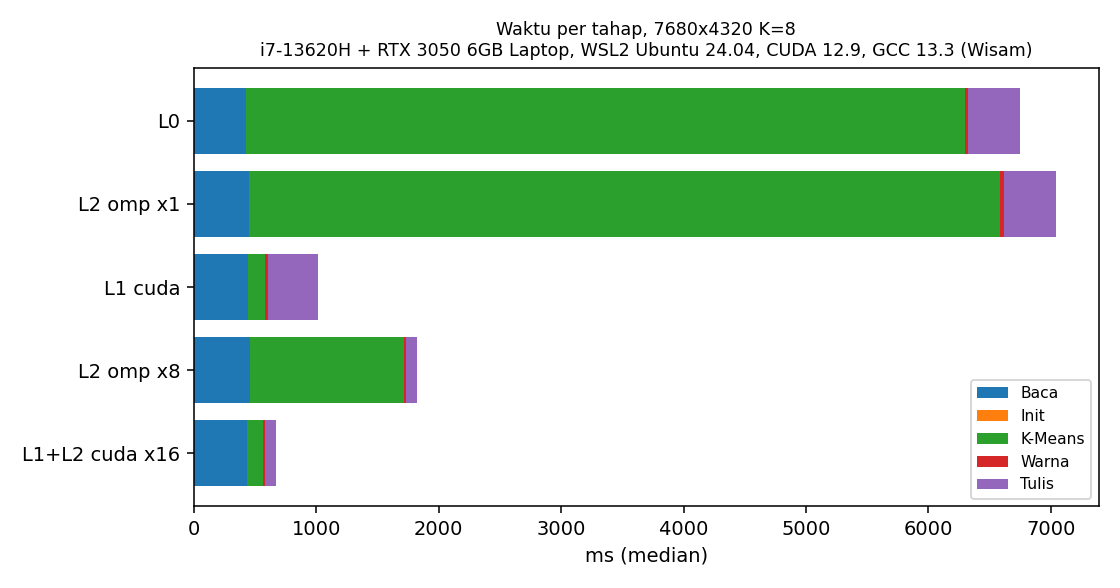
\includegraphics[width=0.92\textwidth]{tahap_7680x4320_k8.png}
\caption{Waktu per tahap pada citra sintetis 7680$\times$4320, $K=8$, Mesin B (median, ms). Sumber: \kode{docs/fig/mesinWisam/}, dibuat \kode{bench/analyze\_scaling.py}}
\label{fig:tahap}
\end{figure}

Pada 7680$\times$4320 dengan $K=8$, Total turun dari \LoTotalDelapan~ms (L0) menjadi \LdLdTotalDelapan~ms pada L1+L2 (\LdLdCfgDelapan), atau \LdLdSTotalDelapan. Kontribusi setiap langkah adalah sebagai berikut:
\begin{itemize}
    \item \textbf{L1 (CUDA).} K-Means turun dari \LoKMDelapan{} menjadi \LdKMDelapan~ms (\LdSKMDelapan), tetapi Total hanya membaik \LdSTotalDelapan. Penyebabnya, waktu di luar K-Means (Total dikurangi K-Means) hampir tidak berubah: \LuarLoDelapan~ms pada L0 dan \LuarLdDelapan~ms pada L1.
    \item \textbf{L2 (OpenMP).} Sendirian, L2 (\LdbCfgDelapan) memberi \LdbSTotalDelapan{} pada Total. Kontribusi terbesarnya justru pada kombinasi dengan L1, karena L2 juga memparalelkan pewarnaan dan tulis PNG.
    \item \textbf{L1+L2.} Waktu di luar K-Means turun menjadi \LuarLdLdDelapan~ms; tulis PNG saja turun dari \TulisLoDelapan{} menjadi \TulisLdLdDelapan~ms. Sisanya didominasi baca PNG (\BacaLdLdDelapan~ms, \PorsiBacaLdLdDelapan{} dari Total), yang tetap serial.
\end{itemize}

% DIBUAT OLEH laporan/skrip/tabel_ke_tex.py -- jangan disunting tangan.
\begin{table}[H]
\centering
\caption{Optimasi bertahap pada 4000$\times$3000 untuk $K=2$, 4, dan 16, citra sintetis, Mesin B (ms; $S$ = \emph{speedup} terhadap L0)}
\label{tab:bertahapk}
\footnotesize
\begin{tabularx}{\textwidth}{L{2.1cm}rL{2.3cm}>{\raggedleft\arraybackslash}X>{\raggedleft\arraybackslash}X>{\raggedleft\arraybackslash}X>{\raggedleft\arraybackslash}X>{\raggedleft\arraybackslash}X>{\raggedleft\arraybackslash}X}
\hline
\hdr{Citra} & \hdr{$K$} & \hdr{Konfigurasi} & \hdr{K-Means} & \hdr{$S$ K-Means} & \hdr{Total} & \hdr{$S$ Total} & \hdr{Proses} & \hdr{$S$ Proses} \\ \hline
4000$\times$3000 & 2 & L0 & 640,7 & 1,0\ensuremath{\times} & 875,1 & 1,00\ensuremath{\times} & 916,1 & 1,00\ensuremath{\times} \\ \hline
4000$\times$3000 & 2 & L2 (8 thr) & 197,0 & 3,3\ensuremath{\times} & 379,5 & 2,31\ensuremath{\times} & 415,5 & 2,20\ensuremath{\times} \\ \hline
4000$\times$3000 & 2 & L1 & 57,4 & 11,2\ensuremath{\times} & 275,5 & 3,18\ensuremath{\times} & 574,3 & 1,60\ensuremath{\times} \\ \hline
4000$\times$3000 & 2 & L1+L2 (4 thr) & 56,3 & 11,4\ensuremath{\times} & 248,7 & 3,52\ensuremath{\times} & 591,0 & 1,55\ensuremath{\times} \\ \hline
4000$\times$3000 & 4 & L0 & 1017,2 & 1,0\ensuremath{\times} & 1224,8 & 1,00\ensuremath{\times} & 1258,4 & 1,00\ensuremath{\times} \\ \hline
4000$\times$3000 & 4 & L2 (4 thr) & 302,2 & 3,4\ensuremath{\times} & 490,1 & 2,50\ensuremath{\times} & 516,0 & 2,44\ensuremath{\times} \\ \hline
4000$\times$3000 & 4 & L1 & 59,6 & 17,1\ensuremath{\times} & 314,6 & 3,89\ensuremath{\times} & 642,0 & 1,96\ensuremath{\times} \\ \hline
4000$\times$3000 & 4 & L1+L2 (2 thr) & 56,3 & 18,1\ensuremath{\times} & 249,1 & 4,92\ensuremath{\times} & 466,1 & 2,70\ensuremath{\times} \\ \hline
4000$\times$3000 & 16 & L0 & 4794,6 & 1,0\ensuremath{\times} & 5400,7 & 1,00\ensuremath{\times} & 5509,7 & 1,00\ensuremath{\times} \\ \hline
4000$\times$3000 & 16 & L2 (16 thr) & 684,2 & 7,0\ensuremath{\times} & 927,9 & 5,82\ensuremath{\times} & 1000,7 & 5,51\ensuremath{\times} \\ \hline
4000$\times$3000 & 16 & L1 & 59,7 & 80,3\ensuremath{\times} & 609,9 & 8,86\ensuremath{\times} & 890,2 & 6,19\ensuremath{\times} \\ \hline
4000$\times$3000 & 16 & L1+L2 (16 thr) & 50,5 & 95,0\ensuremath{\times} & 300,6 & 17,97\ensuremath{\times} & 613,4 & 8,98\ensuremath{\times} \\ \hline
\end{tabularx}
\par\smallskip\footnotesize\raggedright Keterangan kolom sama dengan Tabel~\ref{tab:bertahapk8}. Sumber: \kode{run\_20261127\_1634\_ksweep\_summary.csv}.
\end{table}


\textbf{Total dan Proses.} Tabel~\ref{tab:bertahapk} memuat empat nilai $K$ pada 4000$\times$3000, satu-satunya ukuran yang Prosesnya terekam. Menurut Total, L1+L2 selalu paling cepat. Menurut Proses, pemanasan konteks CUDA menutup sebagian besar keuntungan GPU. Pada $K=8$, L1+L2 (\LdLdCfgEmpat) memberi \LdLdSTotalEmpat{} menurut Total tetapi hanya \LdLdSProsesEmpat{} menurut Proses. Konfigurasi Optimalisasi tercepat menurut Proses memberi \emph{speedup} \SProsesTerbaikKDua{} ($K=2$, \CfgProsesTerbaikKDua), \SProsesTerbaikKEmpat{} ($K=4$, \CfgProsesTerbaikKEmpat), \SProsesTerbaikKDelapan{} ($K=8$, \CfgProsesTerbaikKDelapan), dan \SProsesTerbaikKEnambelas{} ($K=16$, \CfgProsesTerbaikKEnambelas). Pada $K=2$, OpenMP tanpa GPU bahkan menjadi pilihan tercepat menurut Proses. Inilah dasar pemilihan mode otomatis (Subbab~\ref{sec:hasilambang}).

\section{\emph{Strong} dan \emph{Weak Scaling} OpenMP}
\label{sec:scaling}
\textbf{\emph{Strong scaling}.} Tabel~\ref{tab:strong} dan Gambar~\ref{fig:strong} memakai OpenMP satu \emph{thread} sebagai basis, bukan L0, agar \emph{overhead} OpenMP tidak tercampur ke dalam efisiensi. \emph{Speedup} K-Means naik sampai 8 \emph{thread} pada semua ukuran, dengan efisiensi yang turun. Dari 8 ke 16 \emph{thread}, hasilnya bergantung pada ukuran dan sesi ukur: 16 \emph{thread} lebih cepat daripada 8 \emph{thread} hanya pada \JmlEnambelasMenang{} dari \JmlStrong{} konfigurasi, yaitu \DaftarEnambelasMenang, yang keduanya berasal dari \emph{run} 16:34. Pada 7680$\times$4320, $K=8$, \emph{speedup} K-Means adalah \StrongDelapanTd{} dengan 8 \emph{thread} dan \StrongDelapanTe{} dengan 16 \emph{thread}. Karena itu, 8 \emph{thread} tidak bisa digeneralisasi sebagai jumlah terbaik, dan 16 \emph{thread} juga tidak.

Penyebab turunnya efisiensi di atas 8 \emph{thread} \textbf{tidak diukur}. Dugaan yang belum diuji: 16 CPU logis di WSL adalah \emph{hyperthread} yang berbagi inti fisik, dan \emph{bandwidth} memori menjadi batas. \emph{Speedup} Total selalu lebih kecil daripada \emph{speedup} K-Means, karena baca PNG serial tidak ikut menskala (Hukum Amdahl, Persamaan~\ref{eq:amdahl}).

% DIBUAT OLEH laporan/skrip/tabel_ke_tex.py -- jangan disunting tangan.
\begin{table}[H]
\centering
\caption{\emph{Strong scaling} OpenMP: \emph{speedup} $S$ terhadap OpenMP 1 \emph{thread} dan efisiensi $E=S/T$, citra sintetis, Mesin B}
\label{tab:strong}
\footnotesize
\begin{tabularx}{\textwidth}{L{2.1cm}r>{\raggedleft\arraybackslash}X>{\raggedleft\arraybackslash}X>{\raggedleft\arraybackslash}X>{\raggedleft\arraybackslash}X>{\raggedleft\arraybackslash}X>{\raggedleft\arraybackslash}X>{\raggedleft\arraybackslash}X>{\raggedleft\arraybackslash}X}
\hline
\hdr{Citra} & \hdr{$K$} & \hdr{K-M $T{=}2$} & \hdr{K-M $T{=}4$} & \hdr{K-M $T{=}8$} & \hdr{K-M $T{=}16$} & \hdr{$E$ K-M $T{=}8$} & \hdr{$E$ K-M $T{=}16$} & \hdr{Total $T{=}8$} & \hdr{Total $T{=}16$} \\ \hline
4000$\times$3000 & 2 & 1,88\ensuremath{\times} & 3,17\ensuremath{\times} & 3,92\ensuremath{\times} & 3,01\ensuremath{\times} & 0,49 & 0,19 & 2,69\ensuremath{\times} & 2,33\ensuremath{\times} \\ \hline
4000$\times$3000 & 4 & 1,72\ensuremath{\times} & 3,73\ensuremath{\times} & 3,86\ensuremath{\times} & 3,00\ensuremath{\times} & 0,48 & 0,19 & 2,61\ensuremath{\times} & 2,25\ensuremath{\times} \\ \hline
1000$\times$1000 & 8 & 1,64\ensuremath{\times} & 4,10\ensuremath{\times} & 5,07\ensuremath{\times} & 2,34\ensuremath{\times} & 0,63 & 0,15 & 3,43\ensuremath{\times} & 1,90\ensuremath{\times} \\ \hline
2000$\times$2000 & 8 & 2,24\ensuremath{\times} & 3,81\ensuremath{\times} & 4,97\ensuremath{\times} & 2,55\ensuremath{\times} & 0,62 & 0,16 & 3,92\ensuremath{\times} & 2,16\ensuremath{\times} \\ \hline
4000$\times$3000 & 8 & 1,90\ensuremath{\times} & 3,39\ensuremath{\times} & 4,72\ensuremath{\times} & 6,83\ensuremath{\times} & 0,59 & 0,43 & 3,82\ensuremath{\times} & 4,89\ensuremath{\times} \\ \hline
7680$\times$4320 & 8 & 2,06\ensuremath{\times} & 3,03\ensuremath{\times} & 4,88\ensuremath{\times} & 4,34\ensuremath{\times} & 0,61 & 0,27 & 3,78\ensuremath{\times} & 3,49\ensuremath{\times} \\ \hline
4000$\times$3000 & 16 & 1,87\ensuremath{\times} & 3,01\ensuremath{\times} & 4,96\ensuremath{\times} & 6,57\ensuremath{\times} & 0,62 & 0,41 & 4,36\ensuremath{\times} & 5,49\ensuremath{\times} \\ \hline
\end{tabularx}
\par\smallskip\footnotesize\raggedright K-M = tahap K-Means saja; Total = \kode{total\_ms} (termasuk baca PNG serial). Basis = \kode{L2 omp x1}, bukan L0. Sumber: \kode{docs/BENCH\_scaling\_mesin\_wisam.md} bagian 3 (dihitung ulang dari CSV).
\end{table}


\begin{figure}[H]
\centering
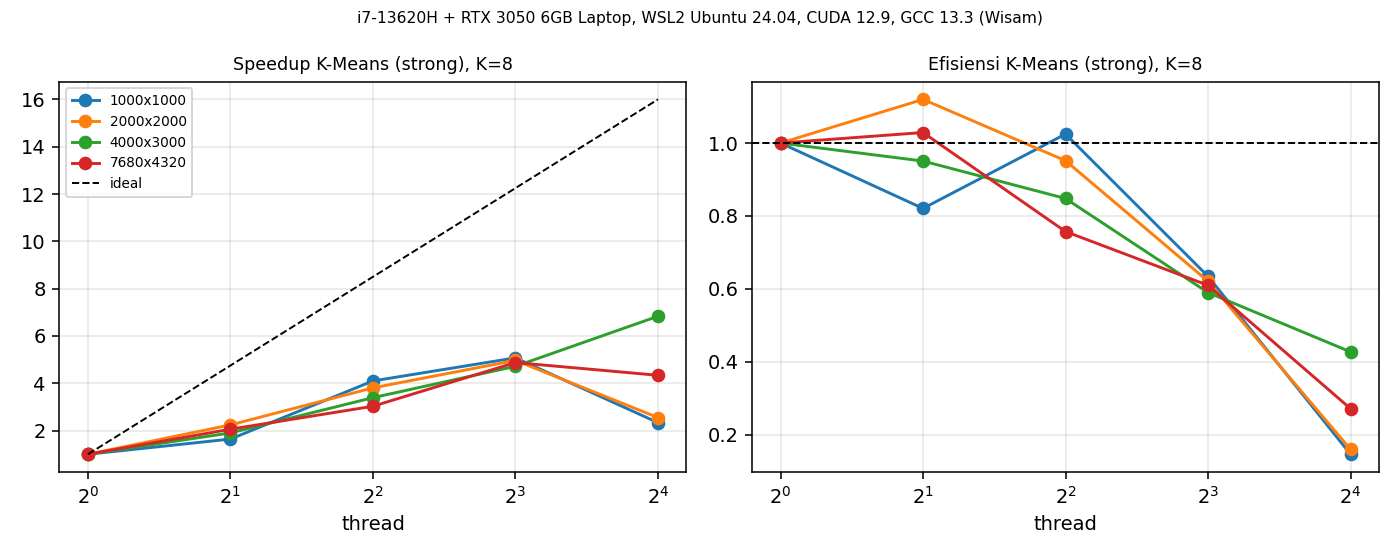
\includegraphics[width=\textwidth]{strong_kmeans_k8.png}
\caption{\emph{Speedup} dan efisiensi K-Means OpenMP (\emph{strong scaling}), $K=8$, citra sintetis, Mesin B. Garis putus-putus = ideal}
\label{fig:strong}
\end{figure}

\textbf{\emph{Weak scaling}.} Pada \emph{weak scaling} (Tabel~\ref{tab:weak}, Gambar~\ref{fig:weak}), beban per \emph{thread} dibuat tetap, sesuai sudut pandang Gustafson \cite{gustafson1988}. Efisiensi K-Means pada $K=8$ masih \WeakKMDua{} dengan 2 \emph{thread}, lalu turun menjadi \WeakKMDelapan{} dengan 8 \emph{thread} dan \WeakKMEnambelas{} dengan 16 \emph{thread}. Efisiensi Total pada 16 \emph{thread} lebih rendah lagi (\WeakTotEnambelas), karena waktu baca PNG serial tumbuh bersama ukuran citra. Jadi menambah \emph{thread} di mesin ini tidak cukup untuk menjaga waktu tetap ketika citra membesar.

% DIBUAT OLEH laporan/skrip/tabel_ke_tex.py -- jangan disunting tangan.
\begin{table}[H]
\centering
\caption{\emph{Weak scaling} OpenMP (beban per \emph{thread} tetap 2 juta piksel), citra sintetis, Mesin B (ms)}
\label{tab:weak}
\footnotesize
\begin{tabularx}{\textwidth}{rL{2.4cm}>{\raggedleft\arraybackslash}X>{\raggedleft\arraybackslash}X>{\raggedleft\arraybackslash}X>{\raggedleft\arraybackslash}X>{\raggedleft\arraybackslash}X>{\raggedleft\arraybackslash}X>{\raggedleft\arraybackslash}X>{\raggedleft\arraybackslash}X}
\hline
\hdr{$T$} & \hdr{Citra} & \hdr{K-M $K{=}4$} & \hdr{$E_w$} & \hdr{Total $K{=}4$} & \hdr{$E_w$} & \hdr{K-M $K{=}8$} & \hdr{$E_w$} & \hdr{Total $K{=}8$} & \hdr{$E_w$} \\ \hline
1 & 2000$\times$1000 & 197,5 & 1,00 & 237,1 & 1,00 & 343,0 & 1,00 & 415,0 & 1,00 \\ \hline
2 & 4000$\times$1000 & 192,4 & 1,03 & 264,0 & 0,90 & 359,0 & 0,96 & 455,1 & 0,91 \\ \hline
4 & 8000$\times$1000 & 257,1 & 0,77 & 389,6 & 0,61 & 461,5 & 0,74 & 626,9 & 0,66 \\ \hline
8 & 16000$\times$1000 & 341,3 & 0,58 & 598,5 & 0,40 & 767,7 & 0,45 & 1100,5 & 0,38 \\ \hline
16 & 32000$\times$1000 & 1038,3 & 0,19 & 1679,0 & 0,14 & 1451,7 & 0,24 & 2148,1 & 0,19 \\ \hline
\end{tabularx}
\par\smallskip\footnotesize\raggedright $E_w = t(T{=}1)/t(T)$, ideal 1. Sumber: \kode{run\_20261127\_1634\_weak\_summary.csv}.
\end{table}


\begin{figure}[H]
\centering
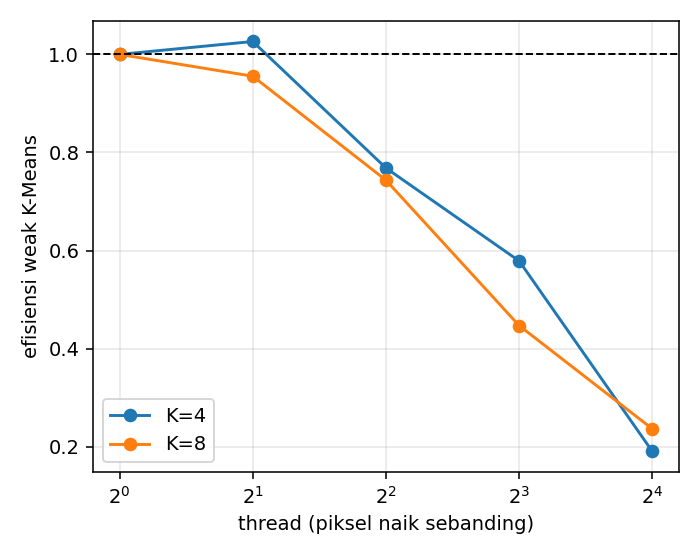
\includegraphics[width=0.55\textwidth]{weak_kmeans.png}
\caption{Efisiensi \emph{weak scaling} K-Means OpenMP, citra sintetis, Mesin B}
\label{fig:weak}
\end{figure}

\section{Kinerja CUDA}
\label{sec:hasilcuda}
\textbf{Rincian waktu.} Tabel~\ref{tab:cudarinci} memecah tahap K-Means CUDA menjadi salin ke GPU (h2d), \emph{kernel}, dan salin kembali (d2h). Pada 7680$\times$4320, $K=8$, rinciannya adalah h2d \HdDelapan~ms, \emph{kernel} \KernelDelapan~ms, dan d2h \DdhDelapan~ms. Pada semua baris, d2h lebih lama daripada h2d (\RasioDdhHdMin--\RasioDdhHdMax). Sebagian selisih ini sesuai dengan ukuran data: label dikirim balik sebagai \kode{int32} (4 \emph{byte} per piksel), sedangkan citra dikirim sebagai 3 \emph{byte} per piksel, atau rasio 4/3. Rasio yang terukur lebih besar daripada itu, dan penyebab sisanya \textbf{tidak diukur} (tanpa Nsight). Transfer hanya terjadi sekali di awal dan sekali di akhir (Subbab~\ref{sec:cuda}), tetapi pada citra besar porsinya tetap besar dibandingkan \emph{kernel} 20 iterasi. Pemanasan konteks CUDA hanya terekam pada 4000$\times$3000; di sana pemanasan lebih lama daripada seluruh tahap K-Means untuk keempat nilai $K$.

% DIBUAT OLEH laporan/skrip/tabel_ke_tex.py -- jangan disunting tangan.
\begin{table}[H]
\centering
\caption{Rincian tahap K-Means CUDA (L1) per citra dan $K$, citra sintetis, Mesin B (ms)}
\label{tab:cudarinci}
\small
\begin{tabularx}{\textwidth}{L{2.3cm}r>{\raggedleft\arraybackslash}X>{\raggedleft\arraybackslash}X>{\raggedleft\arraybackslash}X>{\raggedleft\arraybackslash}X>{\raggedleft\arraybackslash}X}
\hline
\hdr{Citra} & \hdr{$K$} & \hdr{h2d} & \hdr{\emph{Kernel}} & \hdr{d2h} & \hdr{K-Means} & \hdr{Pemanasan} \\ \hline
4000$\times$3000 & 2 & 7,5 & 25,6 & 24,0 & 57,4 & 191 \\ \hline
4000$\times$3000 & 4 & 11,3 & 26,0 & 22,5 & 59,6 & 195 \\ \hline
1000$\times$1000 & 8 & 0,8 & 2,1 & 2,0 & 4,8 & -- \\ \hline
2000$\times$2000 & 8 & 2,9 & 7,7 & 8,0 & 18,5 & -- \\ \hline
4000$\times$3000 & 8 & 7,8 & 23,4 & 24,1 & 55,7 & 194 \\ \hline
7680$\times$4320 & 8 & 21,6 & 53,7 & 62,1 & 138,9 & -- \\ \hline
4000$\times$3000 & 16 & 9,2 & 21,9 & 23,6 & 59,7 & 214 \\ \hline
\end{tabularx}
\par\smallskip\footnotesize\raggedright h2d/\emph{kernel}/d2h diukur dengan CUDA \emph{events}. Pemanasan = inisialisasi konteks CUDA (\kode{warmup\_ms}), di luar \kode{total\_ms}; ``--'' = tidak direkam pada sesi \kode{bench\_gpu}.
\end{table}


\textbf{Pengaruh $K$.} Pada 4000$\times$3000 (Tabel~\ref{tab:pengaruhk}), K-Means L0 tumbuh \RasioKLo{} dari $K=2$ ke $K=16$, mendekati linear terhadap $K$. K-Means CUDA hampir datar (\RasioKCuda). Tabel~\ref{tab:cudarinci} menunjukkan bahwa waktu \emph{kernel} sendiri juga hampir tidak berubah terhadap $K$ (\KernelKMin--\KernelKMax~ms untuk $K=2$ sampai 16). Dugaan yang \textbf{tidak diukur}: \emph{kernel} dibatasi akses memori (membaca citra dan menulis label), bukan perhitungan jarak yang sebanding dengan $K$. Akibatnya, \emph{speedup} K-Means CUDA membesar bersama $K$ dan mencapai \LdSKMEnambelas{} pada $K=16$.

% DIBUAT OLEH laporan/skrip/tabel_ke_tex.py -- jangan disunting tangan.
\begin{table}[H]
\centering
\caption{Waktu K-Means (ms) terhadap $K$ pada 4000$\times$3000, citra sintetis, Mesin B (dalam kurung: rasio terhadap $K=2$)}
\label{tab:pengaruhk}
\small
\begin{tabularx}{\textwidth}{L{2.6cm}>{\raggedleft\arraybackslash}X>{\raggedleft\arraybackslash}X>{\raggedleft\arraybackslash}X>{\raggedleft\arraybackslash}X}
\hline
\hdr{Konfigurasi} & \hdr{$K=2$} & \hdr{$K=4$} & \hdr{$K=8$} & \hdr{$K=16$} \\ \hline
L0 & 640,7 (1,00\ensuremath{\times}) & 1017,2 (1,59\ensuremath{\times}) & 2385,1 (3,72\ensuremath{\times}) & 4794,6 (7,48\ensuremath{\times}) \\ \hline
L2 (8 thr) & 197,0 (1,00\ensuremath{\times}) & 292,2 (1,48\ensuremath{\times}) & 488,5 (2,48\ensuremath{\times}) & 907,0 (4,61\ensuremath{\times}) \\ \hline
L2 (16 thr) & 256,7 (1,00\ensuremath{\times}) & 376,1 (1,46\ensuremath{\times}) & 337,3 (1,31\ensuremath{\times}) & 684,2 (2,67\ensuremath{\times}) \\ \hline
L1 & 57,4 (1,00\ensuremath{\times}) & 59,6 (1,04\ensuremath{\times}) & 55,7 (0,97\ensuremath{\times}) & 59,7 (1,04\ensuremath{\times}) \\ \hline
L1+L2 (8 thr) & 63,5 (1,00\ensuremath{\times}) & 69,6 (1,09\ensuremath{\times}) & 55,4 (0,87\ensuremath{\times}) & 53,7 (0,84\ensuremath{\times}) \\ \hline
\end{tabularx}
\par\smallskip\footnotesize\raggedright Sumber: \kode{run\_20261127\_1634\_ksweep\_summary.csv}.
\end{table}


\textbf{\emph{Throughput}.} Tabel~\ref{tab:throughput} menunjukkan bahwa CUDA memproses \TpCudaMin--\TpCudaMax~ns per piksel per iterasi pada $K=8$ di semua ukuran. Angka yang datar ini berarti waktu K-Means CUDA tumbuh linear terhadap jumlah piksel pada rentang yang diukur.

% DIBUAT OLEH laporan/skrip/tabel_ke_tex.py -- jangan disunting tangan.
\begin{table}[H]
\centering
\caption{\emph{Throughput} K-Means dalam ns per piksel per iterasi, $K=8$, citra sintetis, Mesin B}
\label{tab:throughput}
\small
\begin{tabularx}{\textwidth}{L{2.6cm}>{\raggedleft\arraybackslash}X>{\raggedleft\arraybackslash}X>{\raggedleft\arraybackslash}X>{\raggedleft\arraybackslash}X}
\hline
\hdr{Citra} & \hdr{Piksel (juta)} & \hdr{L0} & \hdr{L2 (8 thr)} & \hdr{L1} \\ \hline
1000$\times$1000 & 1,00 & 10,37 & 2,17 & 0,24 \\ \hline
2000$\times$2000 & 4,00 & 9,72 & 2,06 & 0,23 \\ \hline
4000$\times$3000 & 12,00 & 9,94 & 2,04 & 0,23 \\ \hline
7680$\times$4320 & 33,18 & 8,85 & 1,90 & 0,21 \\ \hline
\end{tabularx}
\par\smallskip\footnotesize\raggedright ns/piksel/iterasi = \kode{kmeans\_ms}$\times10^6$/(piksel$\times$iterasi). Sumber: \kode{docs/BENCH\_scaling\_mesin\_wisam.md} bagian 5 (dihitung ulang dari CSV).
\end{table}


\textbf{Varian \emph{kernel}.} Tabel~\ref{tab:variancuda} membandingkan tiga varian pada tahap K-Means saja, diukur dengan \kode{tests/bench\_cuda} di luar \kode{landcover}. Reduksi di \emph{shared memory} (T4) \TempatTigaMin--\TempatTigaMax{} lebih cepat daripada \kode{atomicAdd} global (T3). Hasil ini sesuai dengan alasan rancangan T4 (Subbab~\ref{sec:cuda}): pada T3 semua \emph{thread} menulis ke akumulator global yang sama, sedangkan T4 menjumlahkan dulu per \emph{block}. Penyebab ini tidak diprofilkan. Varian \emph{streams} dengan \emph{pinned memory} (T5) \LimaEmpatMin--\LimaEmpatMax{} lebih lambat daripada T4 pada semua ukuran yang diukur. Dugaan yang \textbf{tidak diukur}: tumpang tindih transfer pada T5 hanya terjadi di iterasi pertama dan terakhir (Subbab~\ref{sec:bersamaan}), sehingga keuntungannya tidak menutup biaya pembagian potongan dan sinkronisasi \emph{stream}. Pengaruh T5 pada \emph{pipeline} utuh \textbf{tidak diukur}, karena \kode{landcover} hanya memanggil T4.

% DIBUAT OLEH laporan/skrip/tabel_ke_tex.py -- jangan disunting tangan.
\begin{table}[H]
\centering
\caption{Varian CUDA pada tahap K-Means saja (\kode{tests/bench\_cuda}, citra acak), Mesin B (ms)}
\label{tab:variancuda}
\small
\begin{tabularx}{\textwidth}{L{2.3cm}r>{\raggedleft\arraybackslash}X>{\raggedleft\arraybackslash}X>{\raggedleft\arraybackslash}X>{\raggedleft\arraybackslash}X>{\raggedleft\arraybackslash}X}
\hline
\hdr{Ukuran} & \hdr{$K$} & \hdr{T3 \emph{simple}} & \hdr{T4 \emph{shared}} & \hdr{T5 \emph{streams}} & \hdr{T4 vs T3} & \hdr{T5 vs T3} \\ \hline
1000$\times$1000 & 4 & 48,0 & 2,8 & 4,2 & 16,9\ensuremath{\times} & 11,4\ensuremath{\times} \\ \hline
1000$\times$1000 & 8 & 39,6 & 3,0 & 3,7 & 13,2\ensuremath{\times} & 10,6\ensuremath{\times} \\ \hline
1000$\times$1000 & 16 & 29,1 & 3,1 & 4,3 & 9,5\ensuremath{\times} & 6,7\ensuremath{\times} \\ \hline
2000$\times$2000 & 8 & 154,1 & 9,7 & 11,6 & 15,9\ensuremath{\times} & 13,3\ensuremath{\times} \\ \hline
4000$\times$3000 & 4 & 450,8 & 30,3 & 39,8 & 14,9\ensuremath{\times} & 11,3\ensuremath{\times} \\ \hline
4000$\times$3000 & 8 & 462,6 & 30,6 & 43,6 & 15,1\ensuremath{\times} & 10,6\ensuremath{\times} \\ \hline
4000$\times$3000 & 16 & 317,4 & 31,5 & 40,7 & 10,1\ensuremath{\times} & 7,8\ensuremath{\times} \\ \hline
7680$\times$4320 & 4 & 1233,5 & 91,3 & 96,4 & 13,5\ensuremath{\times} & 12,8\ensuremath{\times} \\ \hline
7680$\times$4320 & 8 & 1277,8 & 98,1 & 101,0 & 13,0\ensuremath{\times} & 12,7\ensuremath{\times} \\ \hline
7680$\times$4320 & 16 & 888,0 & 89,6 & 95,6 & 9,9\ensuremath{\times} & 9,3\ensuremath{\times} \\ \hline
\end{tabularx}
\par\smallskip\footnotesize\raggedright Diukur di luar \kode{landcover} (tanpa baca/tulis PNG). Sumber: \kode{run\_20261127\_1634\_cudavar\_summary.csv}.
\end{table}


\section{Ambang Mode Otomatis}
\label{sec:hasilambang}
Tabel~\ref{tab:ambang} membandingkan OpenMP dan CUDA pada \AmbJumlah{} konfigurasi (citra sintetis $N$ sampai \AmbNMax{} juta piksel, $K$ = 4, 8, 16). Menurut Total, CUDA unggul pada \AmbCudaTotal{} dari \AmbJumlah{} konfigurasi. Menurut Proses, CUDA hanya unggul pada \AmbCudaProses{} konfigurasi, karena pemanasan konteks CUDA (\AmbWarmMin--\AmbWarmMax~ms pada sesi ini) lebih besar daripada keuntungan K-Means pada citra kecil dan $K$ kecil.

% DIBUAT OLEH laporan/skrip/tabel_ke_tex.py -- jangan disunting tangan.
\begin{table}[H]
\centering
\caption{Pemenang OpenMP vs CUDA menurut Total dan menurut Proses pada 21 konfigurasi, citra sintetis, Mesin B (ms)}
\label{tab:ambang}
\footnotesize
\begin{tabularx}{\textwidth}{rr>{\raggedleft\arraybackslash}X>{\raggedleft\arraybackslash}X>{\raggedleft\arraybackslash}X>{\raggedleft\arraybackslash}X>{\raggedleft\arraybackslash}X>{\raggedleft\arraybackslash}X>{\raggedleft\arraybackslash}X>{\raggedleft\arraybackslash}X}
\hline
\hdr{$N$ (juta)} & \hdr{$K$} & \hdr{$N{\times}K$ (juta)} & \hdr{omp Total} & \hdr{cuda Total} & \hdr{Unggul} & \hdr{omp Proses} & \hdr{cuda Proses} & \hdr{Unggul} & \hdr{Aturan} \\ \hline
0,10 & 4 & 0,4 & 7,0 & 4,6 & cuda & 40,6 & 291,3 & omp & omp \\ \hline
0,41 & 4 & 1,6 & 20,2 & 11,2 & cuda & 43,9 & 268,3 & omp & omp \\ \hline
1,00 & 4 & 4,0 & 40,9 & 26,1 & cuda & 68,1 & 265,1 & omp & omp \\ \hline
4,00 & 4 & 16,0 & 168,0 & 87,4 & cuda & 207,0 & 351,9 & omp & omp \\ \hline
6,25 & 4 & 25,0 & 231,0 & 138,3 & cuda & 267,1 & 554,8 & omp & omp \\ \hline
9,00 & 4 & 36,0 & 333,8 & 187,0 & cuda & 370,1 & 447,9 & omp & omp \\ \hline
12,00 & 4 & 48,0 & 432,5 & 248,1 & cuda & 469,9 & 554,0 & omp & omp \\ \hline
0,10 & 8 & 0,8 & 10,2 & 5,9 & cuda & 39,4 & 251,2 & omp & omp \\ \hline
0,41 & 8 & 3,3 & 34,9 & 19,3 & cuda & 71,1 & 278,8 & omp & omp \\ \hline
1,00 & 8 & 8,0 & 70,7 & 37,6 & cuda & 112,1 & 303,6 & omp & omp \\ \hline
4,00 & 8 & 32,0 & 242,6 & 105,8 & cuda & 298,7 & 398,7 & omp & omp \\ \hline
6,25 & 8 & 50,0 & 371,6 & 153,9 & cuda & 421,3 & 444,6 & omp & omp \\ \hline
9,00 & 8 & 72,0 & 538,3 & 218,1 & cuda & 601,7 & 517,6 & cuda & cuda \\ \hline
12,00 & 8 & 96,0 & 703,5 & 276,1 & cuda & 765,0 & 599,7 & cuda & cuda \\ \hline
0,10 & 16 & 1,6 & 14,3 & 5,8 & cuda & 36,0 & 230,6 & omp & omp \\ \hline
0,41 & 16 & 6,6 & 56,6 & 23,0 & cuda & 100,4 & 296,1 & omp & omp \\ \hline
1,00 & 16 & 16,0 & 131,0 & 50,8 & cuda & 203,3 & 319,3 & omp & omp \\ \hline
4,00 & 16 & 64,0 & 421,3 & 124,2 & cuda & 496,0 & 573,8 & omp & omp \\ \hline
6,25 & 16 & 100,0 & 627,4 & 171,2 & cuda & 696,7 & 506,3 & cuda & cuda \\ \hline
9,00 & 16 & 144,0 & 896,6 & 247,7 & cuda & 983,5 & 563,0 & cuda & cuda \\ \hline
12,00 & 16 & 192,0 & 1151,2 & 305,5 & cuda & 1224,7 & 658,3 & cuda & cuda \\ \hline
\end{tabularx}
\par\smallskip\footnotesize\raggedright omp = \kode{L2 omp x8}; cuda = yang tercepat dari L1 dan L1+L2 (8 \emph{thread}) untuk kriteria itu. Proses = waktu dinding, termasuk pemanasan CUDA. Aturan = pilihan $N\times K\geq70$ juta. Sumber: \kode{bench/results/ambang\_summary.csv} (\kode{bench/fit\_auto\_threshold.py}).
\end{table}


Aturan yang diuji:
\begin{itemize}
    \item \textbf{Aturan lama} ($N\geq100.000$ piksel, diturunkan dari Total) memilih yang tercepat menurut Proses hanya pada \AmbLamaBenarProses{} dari \AmbJumlah{} konfigurasi, dengan kerugian \AmbLamaRugi~ms.
    \item \textbf{Selalu OpenMP} benar pada \AmbOmpBenarProses{} konfigurasi, dengan kerugian \AmbOmpRugi~ms.
    \item \textbf{Aturan baru} $N\times K\geq70$ juta (Persamaan~\ref{eq:ambang}) benar pada \AmbBaruBenarProses{} dari \AmbJumlah{} konfigurasi, dengan kerugian \AmbBaruRugi~ms.
\end{itemize}
Aturan baru memakai $N\times K$, bukan $N$ saja, karena waktu K-Means OpenMP sebanding dengan $N\times K$, sedangkan K-Means CUDA hampir tidak bergantung pada $K$ (Tabel~\ref{tab:pengaruhk}). Aturan ini hanya berlaku untuk mesin, data, dan cara pemanggilan yang diukur. Bila aplikasi kelak memakai proses CUDA yang menetap, sehingga pemanasan dibayar sekali, ambang harus dihitung ulang dengan Total.

\section{Verifikasi Hasil Identik}
\label{sec:hasilverifikasi}
Tabel~\ref{tab:verifikasi} merangkum semua pemeriksaan kesamaan hasil antarmode. Pemeriksaan pada kolom ``Identik'' \emph{benchmark} hanya membandingkan \emph{centroid} dan \emph{counts}. Kesamaan label per piksel dibuktikan oleh program uji inti dan oleh \kode{cmp} pada \kode{labels.u8}.

\begin{table}[H]
\centering
\caption{Ringkasan verifikasi hasil identik antarmode}
\label{tab:verifikasi}
\small
\begin{tabularx}{\textwidth}{L{3.3cm}YL{3.4cm}L{2.5cm}}
\hline
\hdr{Uji} & \hdr{Yang dibandingkan} & \hdr{Cakupan} & \hdr{Hasil} \\ \hline
\kode{test\_ref} & Implementasi acuan C++ & Kasus uji inti & 0 kegagalan \\ \hline
\kode{test\_cuda\_vs\_ref} & Label dan \emph{centroid} CUDA vs serial & 615 kasus (ukuran, $K$, \emph{seed}) & 615 dari 615 lulus \\ \hline
\kode{test\_omp\_vs\_cpu} & Label dan \emph{centroid} OpenMP vs serial & Kasus uji OpenMP & Semua sama \\ \hline
\kode{test\_png\_omp} & PNG paralel vs serial & Berkas PNG keluaran & Lulus (\emph{exit} 0) \\ \hline
Kolom ``Identik'' \emph{benchmark} & \emph{Centroid} dan \emph{counts} vs L0 & \IdentikJumlah{} baris ringkasan \emph{benchmark} Mesin B (sintetis) & \IdentikYa{} dari \IdentikJumlah{} identik \\ \hline
\kode{cmp} Sentinel-2 (25 Nov) & \kode{labels.u8}, \emph{centroid}, \emph{counts}: cpu vs cuda & 512, 1024, 2048 px $\times$ $K$ = 4, 8, 16 & 9 dari 9 identik \\ \hline
\kode{cmp} Sentinel-2 (28 Nov) & \kode{labels.u8}, \emph{centroid}, \emph{counts}: cpu vs omp dan cpu vs cuda & 2048 px, $K=8$, biner \kode{main} & \CmpSama{} dari \CmpSama{} berkas identik \\ \hline
Aplikasi (halaman Kinerja) & \kode{labels.u8} penuh, \emph{centroid}, \emph{counts} & Sentinel-2 2048 px, $K=8$ & ``Label identik 100\%'' \\ \hline
\kode{pytest} (Windows) & Logika aplikasi & Seluruh \emph{suite} & 1000 lulus, 41 dilewati, 1 gagal* \\ \hline
Tes biner nyata & Aplikasi + \kode{landcover} asli & Lewat pembungkus WSL & 36 lulus, 3 dilewati \\ \hline
\end{tabularx}
\par\smallskip\footnotesize\raggedright *Tes batas waktu 1 detik yang peka beban mesin; diulang tersendiri, lulus 3 dari 3. Tes yang dilewati hanya berlaku bila OpenMP/CUDA \emph{tidak} terhubung. Sumber: uji 28 Nov pada \kode{main} \kode{f78b5d4} (Mesin C), \kode{bench/results/*\_summary.csv}, dan \kode{laporan/hasil\_s2/cmp.txt}.
\end{table}

Hasilnya identik pada semua pemeriksaan. Ini sesuai rancangan pada Subbab~\ref{sec:konsistensi}: aritmetika integer, pembagian dibulatkan ke bawah, aturan seri yang sama, dan \emph{centroid} awal yang dihitung sekali di CPU. Karena labelnya identik, persentase dan luas setiap kelas pada kedua mode juga identik, dan selisih waktu di subbab sebelumnya murni berasal dari optimasi.

\section{Hasil Aplikasi pada Sentinel-2}
\label{sec:hasilsentinel}
Gambar~\ref{fig:s2peta} menampilkan potongan Sentinel-2 T49MDM 2048$\times$2048 piksel (\SPiksel{} piksel) dan peta kelompok hasil K-Means dengan $K=8$, 20 iterasi, dan \emph{seed} 42. Peta ini dibuat oleh \kode{landcover} versi \kode{main}; mode cpu, omp, dan cuda menghasilkan \kode{labels.u8} yang identik (Tabel~\ref{tab:verifikasi}). Sebanyak \SNodataPiksel{} piksel (\SNodataPersen) adalah \emph{nodata} $(0,0,0)$ pada baji di tepi kanan potongan. Seluruh piksel itu jatuh ke kelompok \SKelompokNodata{} dan dikecualikan dari persen dan luas.

\begin{figure}[H]
\centering
\begin{minipage}{0.48\textwidth}\centering
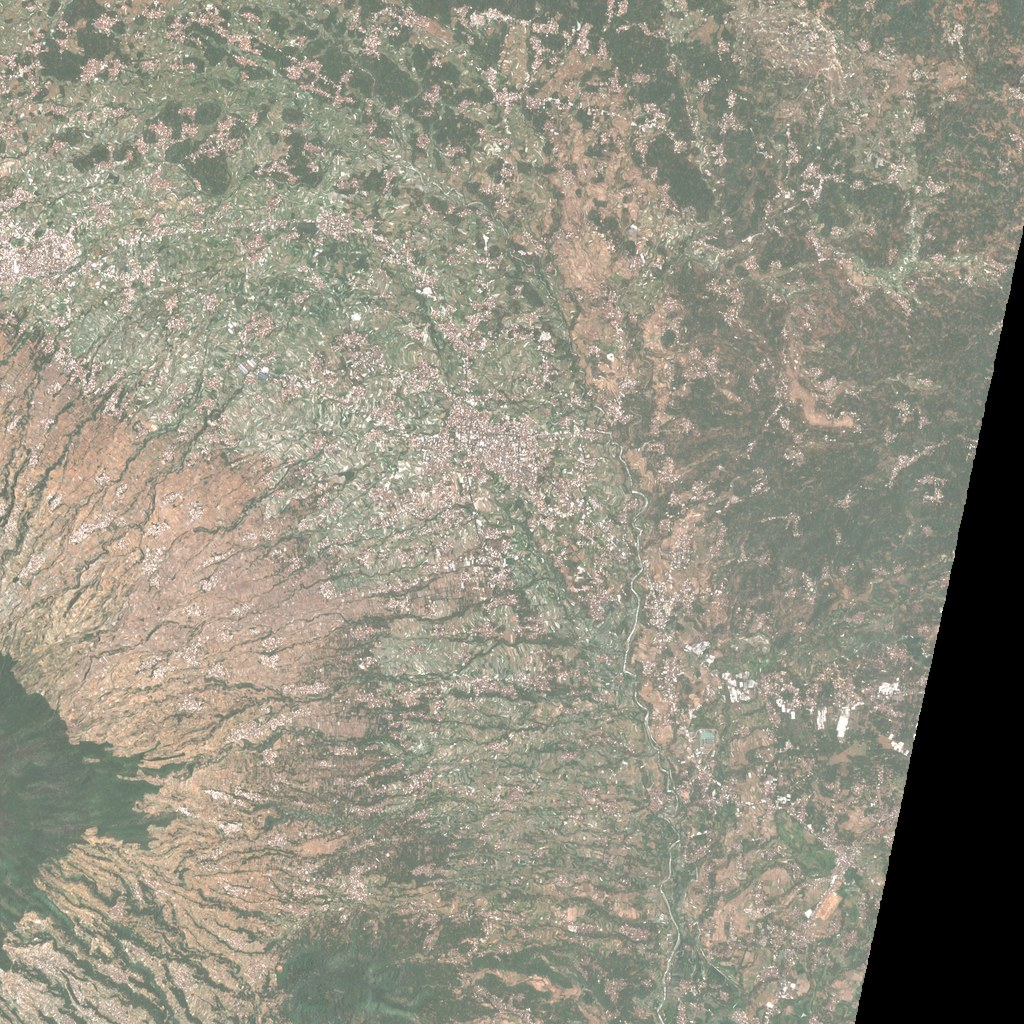
\includegraphics[width=\textwidth]{s2_mdm2048_asli.jpg}\\[2pt]
\small (a) Citra asli (B04/B03/B02)
\end{minipage}\hfill
\begin{minipage}{0.48\textwidth}\centering
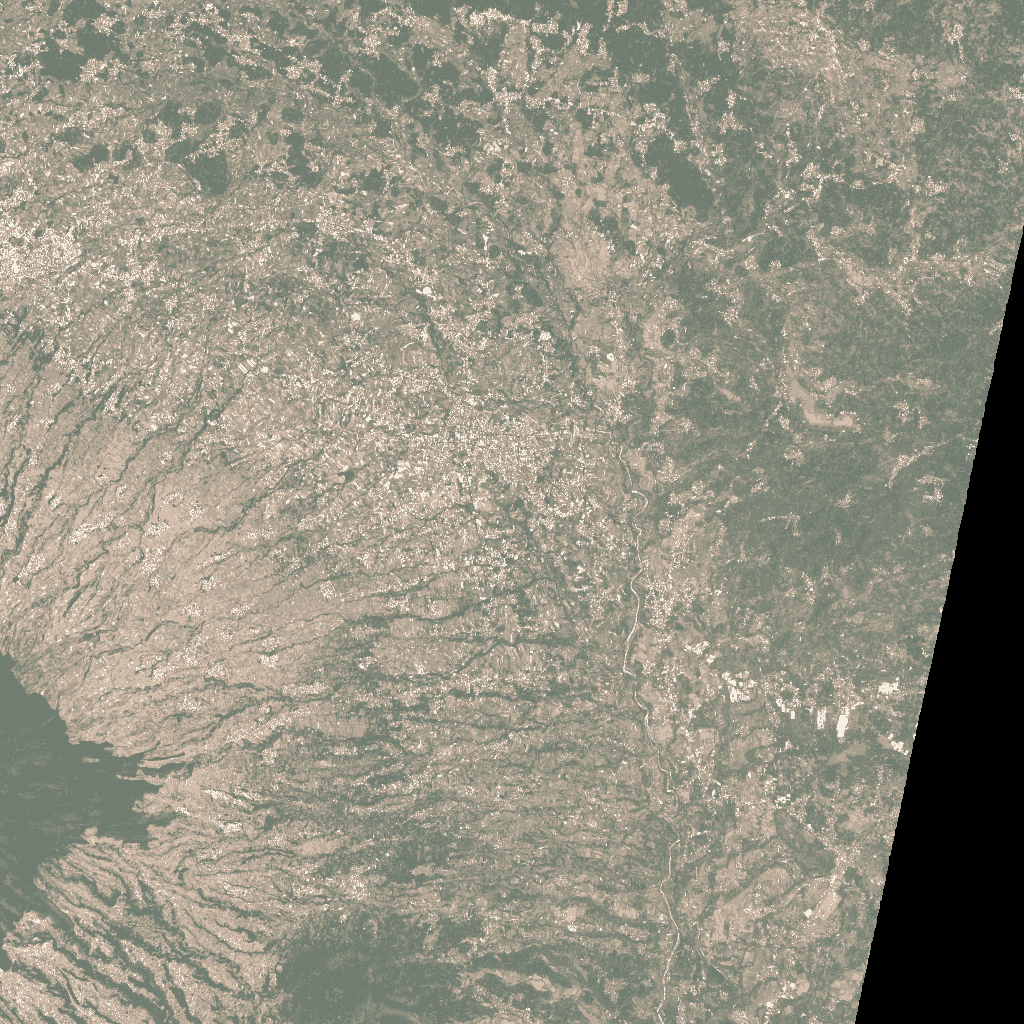
\includegraphics[width=\textwidth]{s2_mdm2048_peta_k8.png}\\[2pt]
\small (b) Peta kelompok, $K=8$
\end{minipage}
\caption{Sentinel-2 T49MDM 2048$\times$2048 px dan peta hasil K-Means. Setiap piksel diwarnai dengan warna \emph{centroid} kelompoknya; gambar diperkecil menjadi 1024 px untuk laporan}
\label{fig:s2peta}
\end{figure}

Tabel~\ref{tab:luass2} menunjukkan persentase dan luas setelah delapan kelompok diberi nama dan digabung menjadi empat kelas di halaman Pemetaan. Total luas valid adalah \SValidHa~ha. Penamaan ini dilakukan manual dari warna \emph{centroid} dan kenampakan visual, sehingga tabel ini adalah contoh keluaran aplikasi, bukan hasil klasifikasi yang tervalidasi.

% DIBUAT OLEH laporan/skrip/tabel_ke_tex.py -- jangan disunting tangan.
\begin{table}[H]
\centering
\caption{Persentase dan luas per kelas, Sentinel-2 T49MDM 2048$\times$2048 px, $K=8$}
\label{tab:luass2}
\small
\begin{tabularx}{\textwidth}{L{2.9cm}Y>{\raggedleft\arraybackslash}p{2.1cm}>{\raggedleft\arraybackslash}p{1.6cm}>{\raggedleft\arraybackslash}p{1.9cm}}
\hline
\hdr{Kelas} & \hdr{Kelompok (\emph{centroid} R,G,B)} & \hdr{Piksel} & \hdr{Persen} & \hdr{Luas (ha)} \\ \hline
Vegetasi & 2 (114,125,113), 5 (126,134,120), 6 (144,145,129) & 1.945.270 & 49,58\% & 19.452,70 \\ \hline
Lahan terbuka & 0 (186,170,153), 3 (211,191,172) & 1.074.523 & 27,38\% & 10.745,23 \\ \hline
Lahan terbangun & 1 (246,239,228) & 114.105 & 2,91\% & 1.141,05 \\ \hline
Lainnya & 4 (164,157,140) & 789.986 & 20,13\% & 7.899,86 \\ \hline
\textbf{Total valid} &  & 3.923.884 & 100,00\% & 39.238,84 \\ \hline
\emph{Nodata} (dikecualikan) & 7 (0,0,0) & 270.420 & 6,45\% & 2.704,20 \\ \hline
\end{tabularx}
\par\smallskip\footnotesize\raggedright Persen kelas dihitung dari piksel valid; persen \emph{nodata} dari seluruh citra. 1 piksel = 10 m $\times$ 10 m. Nama kelas diberikan manual dari warna \emph{centroid} dan kenampakan visual (bukan klasifikasi terverifikasi). Sumber: \kode{laporan/hasil\_s2/} (\kode{counts.json}, \kode{meta\_cpu.json}, \kode{kelas.json}); Mesin C.
\end{table}


Beberapa kasus sulit terlihat karena hanya tiga kanal tampak yang dipakai (tanpa NIR/SWIR):
\begin{enumerate}
    \item \textbf{Air dan bayangan.} Pada $K=8$ tidak terbentuk kelompok air tersendiri. Koridor sungai dan bayangan lereng masuk ke kelompok vegetasi gelap (kelompok 2 dan 5), sehingga kelas Air tidak dibuat.
    \item \textbf{Permukiman dan tanah terbuka.} Atap terang (kelompok 1) berdekatan secara spektral dengan tanah kering dan kabut tipis (kelompok 3). Kelompok 4 mencampur lahan terasering, jalan, dan tepi vegetasi, sehingga diberi nama ``Lainnya''.
    \item \textbf{Kelompok kosong.} Pada $K=16$ dengan \emph{seed} yang sama, beberapa \emph{centroid} awal jatuh pada piksel \emph{nodata} $(0,0,0)$. Tiga \emph{centroid} awal bernilai $(0,0,0)$; dua di antaranya (kelompok 9 dan 12) berakhir dengan nol piksel, sehingga kelompok bukan-\emph{nodata} yang berisi tinggal 13, bukan 15. Perilaku ini sah menurut kontrak (kelompok kosong dipertahankan dan ditampilkan 0\%), tetapi menunjukkan bahwa \emph{nodata} sebaiknya dikeluarkan sebelum inisialisasi bila hasil $K$ besar dibutuhkan.
\end{enumerate}

Waktu \emph{run} Sentinel-2 di Mesin C tidak dilaporkan sebagai hasil kinerja, karena hanya berupa uji fungsional (satu \emph{run} per konfigurasi, mesin berbeda, citra lebih kecil daripada citra pengukuran utama).

\section{Hipotesis dan Analisis Amdahl}
\label{sec:hipotesis}
Tabel~\ref{tab:hipotesis} membandingkan hipotesis Subbab~\ref{sec:hipotesisawal} dengan data terdekat dari Mesin B.

\begin{table}[H]
\centering
\caption{Hipotesis dan hasil pengukuran (Mesin B, citra sintetis, kecuali H4)}
\label{tab:hipotesis}
\small
\begin{tabularx}{\textwidth}{L{3.2cm}YL{3.5cm}}
\hline
\hdr{Hipotesis} & \hdr{Data terdekat} & \hdr{Kesimpulan} \\ \hline
H1: K-Means mengambil porsi terbesar pada L0 & Porsi K-Means \PorsiKMLoMin--\PorsiKMLoMax{} di Mesin B (Tabel~\ref{tab:l0b}) dan \PorsiKMAMin--\PorsiKMAMax{} di Mesin A (Tabel~\ref{tab:l0a}) & Terbukti pada kedua mesin \\ \hline
H2a: K-Means CUDA $\geq20\times$ (4096$^2$, $K=8$) & 4096$^2$ tidak diukur. Ukuran terdekat 4000$\times$3000 (12 juta piksel, bukan 16,8 juta): \LdSKMEmpat. Semua ukuran $K=8$: \HDuaCudaMin--\HDuaCudaMax{} (Tabel~\ref{tab:bertahapk8}) & Tercapai pada ukuran terdekat \\ \hline
H2b: K-Means OpenMP 8 \emph{thread} $\geq4\times$ & Terhadap L0, $K=8$: \HDuaOmpMin--\HDuaOmpMax{} di semua ukuran; terhadap OpenMP 1 \emph{thread} pada 4000$\times$3000: \HDuaOmpSatuEmpat. Pada 4000$\times$3000: $K=2$ \HDuaOmpKDua, $K=4$ \HDuaOmpKEmpat, $K=16$ \HDuaOmpKEnambelas & Tercapai pada $K=8$ (kondisi hipotesis); tidak tercapai pada $K\leq4$ \\ \hline
H3: \emph{End-to-end} satu \emph{tile} penuh $\geq5\times$ & \emph{Tile} penuh tidak diukur. 7680$\times$4320, $K=8$: Total \LdLdSTotalDelapan, Proses tidak diukur. 4000$\times$3000, $K=8$: Total \LdLdSTotalEmpat, Proses \SProsesTerbaikKDelapan{} (konfigurasi tercepat); $K=16$: Proses \SProsesTerbaikKEnambelas & Tidak dapat disimpulkan untuk \emph{tile} penuh. Pada 12 juta piksel, $K=8$: tercapai menurut Total, tidak menurut Proses \\ \hline
H4: Label identik 100\% & \kode{test\_cuda\_vs\_ref}, \kode{test\_omp\_vs\_cpu}, \kode{cmp} \kode{labels.u8} Sentinel-2 cpu vs omp vs cuda (Tabel~\ref{tab:verifikasi}) & Terbukti \\ \hline
\end{tabularx}
\end{table}

\textbf{Analisis Amdahl.} Pada L0 7680$\times$4320, $K=8$, porsi K-Means adalah $q=\AmdP$. Bila hanya K-Means yang dipercepat tanpa batas, Persamaan~\ref{eq:amdahl} dengan fraksi serial $f=1-q$ dan $p\to\infty$ memberi batas \emph{speedup} total $1/(1-q)\approx\AmdBatas$ \cite{amdahl1967}. Hasil pengukuran sesuai dengan analisis ini:
\begin{enumerate}
    \item L1 saja mempercepat K-Means \LdSKMDelapan, tetapi Total hanya membaik \LdSTotalDelapan, mendekati batas \AmdBatas. Tahap lain belum disentuh, sehingga mempercepat K-Means lebih jauh hampir tidak berguna.
    \item L1+L2 mencapai \LdLdSTotalDelapan, melampaui batas tersebut, karena L2 juga memangkas tahap di luar K-Means (pewarnaan dan tulis PNG). Dengan demikian fraksi serialnya mengecil dan batasnya bergeser. Ini menunjukkan mengapa setiap tahap perlu ditempatkan di perangkat terbaiknya, bukan hanya K-Means.
    \item Sesudah L1+L2, K-Means tinggal \PorsiKMLdLdDelapan{} dari Total, sedangkan baca PNG serial menjadi tahap terbesar (\PorsiBacaLdLdDelapan). Bahkan bila K-Means menjadi nol, Total hanya bisa membaik \AmdBatasLdLd{} lagi. Baca PNG adalah \emph{bottleneck} berikutnya.
\end{enumerate}

\section{Batasan}
\label{sec:batasan}
\begin{enumerate}
    \item \textbf{\emph{Tile} penuh tidak diuji.} Data Sentinel-2 yang tersedia hanya potongan sampai 2048 piksel; \emph{tile} 10980$\times$10980 (sekitar 120 juta piksel) tidak ada. Hasil terbesar yang diukur adalah citra sintetis 7680$\times$4320 (sekitar 33 juta piksel), dan H3 tidak dapat disimpulkan untuk \emph{tile} penuh.
    \item \textbf{Kinerja hanya pada citra sintetis.} Waktu baca dan tulis PNG bergantung pada isi citra (kompresi), sehingga angka baca/tulis citra sintetis tidak otomatis berlaku untuk citra satelit.
    \item \textbf{L3 hanya di tingkat \emph{kernel}.} Varian \emph{streams} diukur dengan \kode{tests/bench\_cuda} dan tidak dipanggil \kode{landcover}. Pemrosesan banyak wilayah sekaligus belum dibuat.
    \item \textbf{Proses tidak lengkap.} Waktu dinding proses hanya terekam pada sesi 4000$\times$3000 dan sesi ambang; untuk 1000$^2$, 2000$^2$, dan 7680$\times$4320 hanya Total yang tersedia.
    \item \textbf{Satu mesin acuan dan lima ulangan.} Semua angka kinerja berasal dari satu laptop (Mesin B) dengan skema daya \emph{Balanced} dan median lima ulangan. Dua sesi ukur di mesin yang sama tidak menghasilkan angka yang identik, sehingga selisih kecil antarkonfigurasi (misalnya 8 dan 16 \emph{thread}) belum tentu bermakna.
    \item \textbf{Tanpa Nsight.} Penyebab turunnya efisiensi OpenMP di atas 8 \emph{thread} dan rincian \emph{kernel} CUDA tidak diprofilkan.
    \item \textbf{Segmentasi tanpa pengawasan.} Hasil aplikasi adalah segmentasi awal dari tiga kanal tampak, bukan klasifikasi tutupan lahan yang akurat. Penamaan kelas manual dan tidak divalidasi dengan data lapangan.
\end{enumerate}
